Data processing took place in three stages: (1) the conversion of the optical microscopy videos to $\alpha$ curves for the fitting of Equation \ref{eqn:alpha}; (2) the determination of grain densities from the electron microscopy images for the fitting of \ref{eqn:rho}; and (3) the use of the fitting results to calculate the parameters governing the Te manufacturing process.  Each of these three stages is treated in a subsection below.  All code involved in the calculations may be found in the Github repository linked in Appendix A.

\subsection{JMAK Equation Fitting to Determine $\dot{N}v^2$}

The optical microscopy videos collected during the films' annealing stage were observed to consist of (1) dark regions corresponding to the amorphous phase and (2) regions of greater intensity correponding to the crystalline phase.  Each frame could therefore be converted to its corresponding $\alpha$-value by calculating its average intensity, then normalizing the resulting data to the maximum and minimum average intensities observed during the anneal ($\alpha = 1$ and $\alpha = 0$, respectively).  Several abrupt jumps in average intensity were recorded; this was attributed to automatic intensity rescaling from the imaging system itself.  Fortunately, none of these jumps occured during the main transition region of the curves, allowing the model to be cleanly fit to a rescaled subset of the data.  The selected regions and assigned $\alpha = 0$ rescaling values for each temperature is noted in Figure \ref{fig:jmak_2} of Appendix B.

The actual data fit employed a modified version of the JMAK equation:
%
	\begin{equation}
	\alpha =
	\begin{cases}
		0 & t < t_0 \\
		1 - \exp \left[ -\frac{\pi}{3} \dot{N} v^2 (t-t_0)^3 
			\right] & t_0 \leq t
	\end{cases}
	\end{equation}
%
where the fitting parameter $t_0$ is introduced to reflect variation in the annealing time and the piecewise nature enforces physicality (i.e. $\alpha = 0$ for $t < t_0$).  The nonlinear fitting was performed with the Python package \textit{lmfit}, which also estimated the standard error associated with each of the fitting parameters.  The results of this fitting are summarized in Table \ref{table:jmak_1} and visualized in Figure \ref{fig:jmak_1}.
	

	\begin{figure}[h]
		\centering
		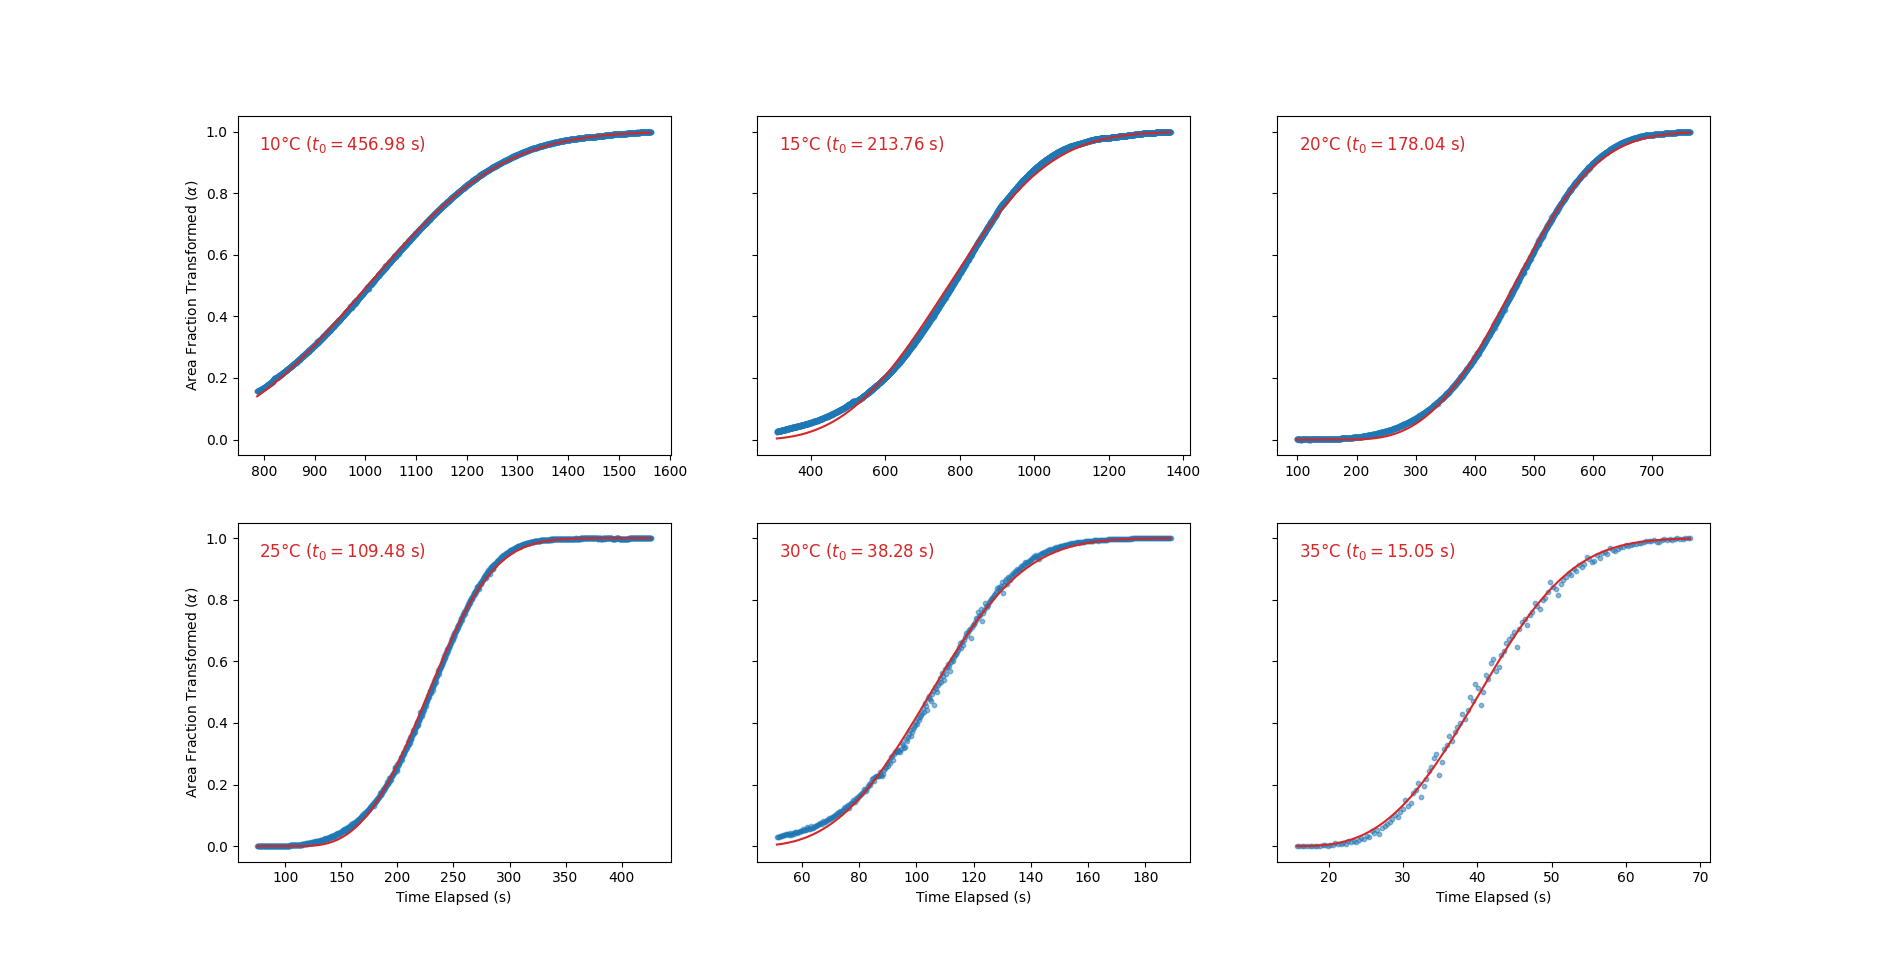
\includegraphics[width=1.0\linewidth]{jmak_1.png}
		\caption{}
		\label{fig:jmak_1}
	\end{figure}

\subsection{Microstructural Image Processing to Determine $\dot{N}/v$}

Using the image analysis procedures described in References \cite{chan:2020} and \cite{campbell:2018} as a loose guide, an rudimentary algorithm was developed in order to process the samples' electron microscopy images and count grains in a consistent manner.  For simplicity, counts were only performed for the 140-\textmu{m} images.  Given the dark field image, the bright field image, and a manual input parameter denoting the minimum detectable grain radius ($r_{min}$), the algorithm does the following:

\begin{enumerate}

	\item Both images are converted to greyscale, after which a Sobel filter is applied to the bright field to calculate its local gradient.  This produces maps where bright regions correspond to possible grain boundaries.

	\item The the two maps are adjusted such that the middle 95\% of pixel intensities are mapped across the intensity range [0, 1], so as to increase contrast for the majority of the map pixels.

	\item The maps are averaged and the results inverted.  In the resulting grain map, bright regions correspond to probable grain locations, while dark regions correspond to boundaries.

	\item Gaussian smoothing is applied to remove some noise, after which gaussian sharpening is applied to increase boundary contrast.

	\item Multiple-otsu thresholding is used to sort the pixels into four different intensity bins; this was observed to isolate grains in the fourth bin, even in the presence of faint grain boundaries (assumed to be low-angle grain boundaries).  The fourth bin therefore produces a binarized image of the grains.

	\item A "weighted opening" is executed upon the binarized image.  The pixels are eroded with a radius of $r{min}$ before being dilated with a radius of $r_{min} / 2$.  This has the effect of eliminating all pixels upon repeated cycling.  Intermediate results are stacked, thereby creating a heatmap of the number of opening cycles required to eliminate any pixel.  This has the effect of replacing each pixel with the distance to the nearest grain boundary, albeit in a way that is meant to promote round grains and smooth heatmap topology.

	\item The local maxima of the heatmap (to within radius $r_{min}$) are counted as the locations of grains.

	\item For diagnostic purposes, the watershed algorithm is then used to produce a grain map and assess the quality of the algorithm's result.

\end{enumerate}

This process is illustrated in Figure \ref{fig:algo_ex} for the 20 \textdegree{C} sample, with comparable figures for all other temperatures contained in Appendix B.  The resulting grain densities and $\dot{N}/v$ values, as calculated using Equation \ref{eqn:rho}, are included in Table \ref{table:data_results}.

	\begin{figure}[h]
		\centering
		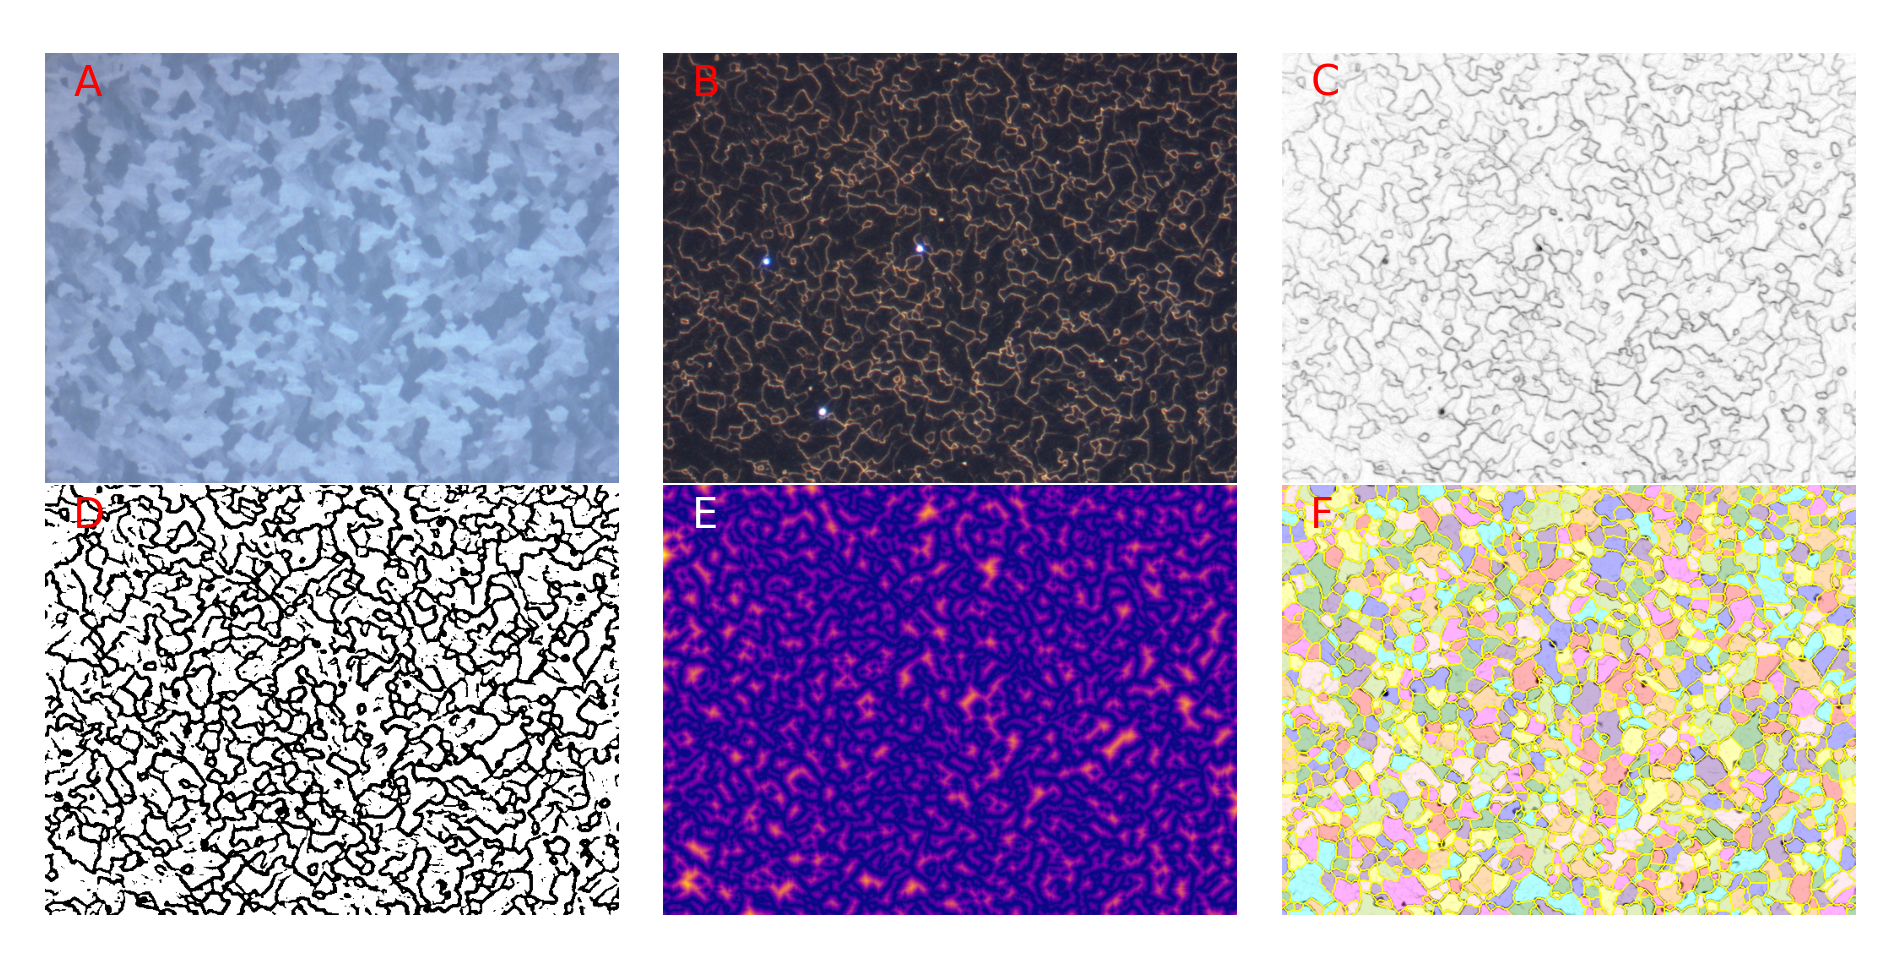
\includegraphics[width=1.0\linewidth]{microstructure_20C.png}
		\caption{}
		\label{fig:algo_ex}
	\end{figure}

A discussion of the quality of the grain-counting algorithm, particularly with respect to the decision not to attempt to quantify its error, is deferred to Section 5.

	\begin{table}[h!]
	\centering
	\begin{tabular}{|c c c c c c c|} 
	\hline
		T (\textdegree{C}) & $\dot{N}v^2 (s^{-3})$ & $\sigma_{\dot{N}v^2}(s^{-3})$ & $t_0 (s)$ & $\sigma_{t_0}$ & $\rho (m^{-2})$ & $\dot{N}/v (m^{-3})$ \\ 
	\hline
		10 & 4.023e-9 & - & 456.98 & - & 3.396e+10 & 7.588e+15\\ 
		15 & 3.845e-9 & - & 213.76 & - & 5.210e+10 & 1.442e+16\\
		20 & 2.773e-8 & 1.115e-10 & 178.04 & 0.427 & 8.469e+10 & 2.989e+16\\
		25 & 3.978e-7 & 2.507e-09 & 109.48 & 0.259 & 9.048e+10 & 3.300e+16\\
		30 & 2.211e-6 & 3.198e-08 & 38.28 & 0.333 & 1.386e+11 & 6.256e+16\\
		35 & 4.069e-5 & 9.426e-7 & 15.05 & 0.201 & 2.644e+11 & 1.648e+17\\
	\hline
	\end{tabular}
		\caption{Summary of results from $\alpha$-fitting (Subsection 4.1) and grain-counting (Subsection 4.2).}
	\label{table:data_results}
	\end{table}

\subsection{Calculation of Crystallization Parameters}

Throughout the following calculations, the standard errors of $\dot{N}v^2$ were propagated according to a well-known formula:

	\begin{equation}
		f(a_1, a_2, ...) \rightarrow \sigma^2_f = \sum_i \left( \frac{\partial f}{\partial a_i} \right)^2 \sigma^2_{a_i}
		\label{eqn:se}
	\end{equation}

From the values of $\dot{N}v^2$ and $\dot{N}/v$ in Table \ref{table:data_results}, $\dot{N}$ and $v$ were obtained for each temperature.  These values are summarized in Table \ref{table:nv_results}:

	\begin{table}[h!]
	\centering
	\begin{tabular}{|c c c c c |} 
	\hline
		T (\textdegree{C}) & $\dot{N}(m^{-2}s^{-1})$ & $\sigma_{\dot{N}}(m^{-2}s^{-1})$ & $v (m/s)$ & $\sigma_{v} (m/s)$ \\ 
	\hline
		10 & 6.141e+07 & - & 8.093651e-09 & -\\ 
		15 & 9.281e+07 & - & 6.436233e-09 & -\\
		20 & 2.915e+08 & 3.907e5 & 9.753040e-09 & 1.307e-11\\
		25 & 7.567e+08 & 1.590e6 & 2.292838e-08 & 4.817e-11\\
		30 & 2.053e+09 & 9.898e6 & 3.281534e-08 & 1.582e-10\\
		35 & 1.034e+10 & 1.983e7 & 6.273605e-08 & 4.843e-10\\
	\hline
	\end{tabular}
		\caption{NV RESULTS}
	\label{table:nv_results}
	\end{table}

These data were then fit to their respective Arrhenius models in ln-versus-$1/T$ coordinates using linear regression so as to estimate the corresponding prefactors and activation energies.  The linear fit is illustrated in Figure \ref{fig:linear_fits}, while the calculated parameters and corresponding standard errors from the linear regression are summarized in Table \ref{table:parameter_results}.  The standard errors of $\dot{N}$ and $v$ were not propagated into this step; all uncertainties stem solely from the linear regression itself.

	\begin{table}[h!]
	\centering
	\begin{tabular}{|c | c | c | c | c |} 
		\hline
		\textbf{Parameter} & $\Delta G(i_c) + \Delta E_{attach}$ (eV) & $\Delta E_{attach}$ (eV) & $\dot{N_0}$ ($m^{-2}s^{-1}$) & $v_0$ (m/s) \\ 
		\hline
		\textbf{Value} & 1.536 & 0.682 & 8.646e34 & 7432 \\
		\textbf{$\sigma$} & 0.136 & 0.117 & 4.615e35 & 34307 \\
		\hline
	\end{tabular}
		\caption{NV RESULTS}
	\label{table:parameter_results}
	\end{table}

	\begin{figure}[h]
		\centering
		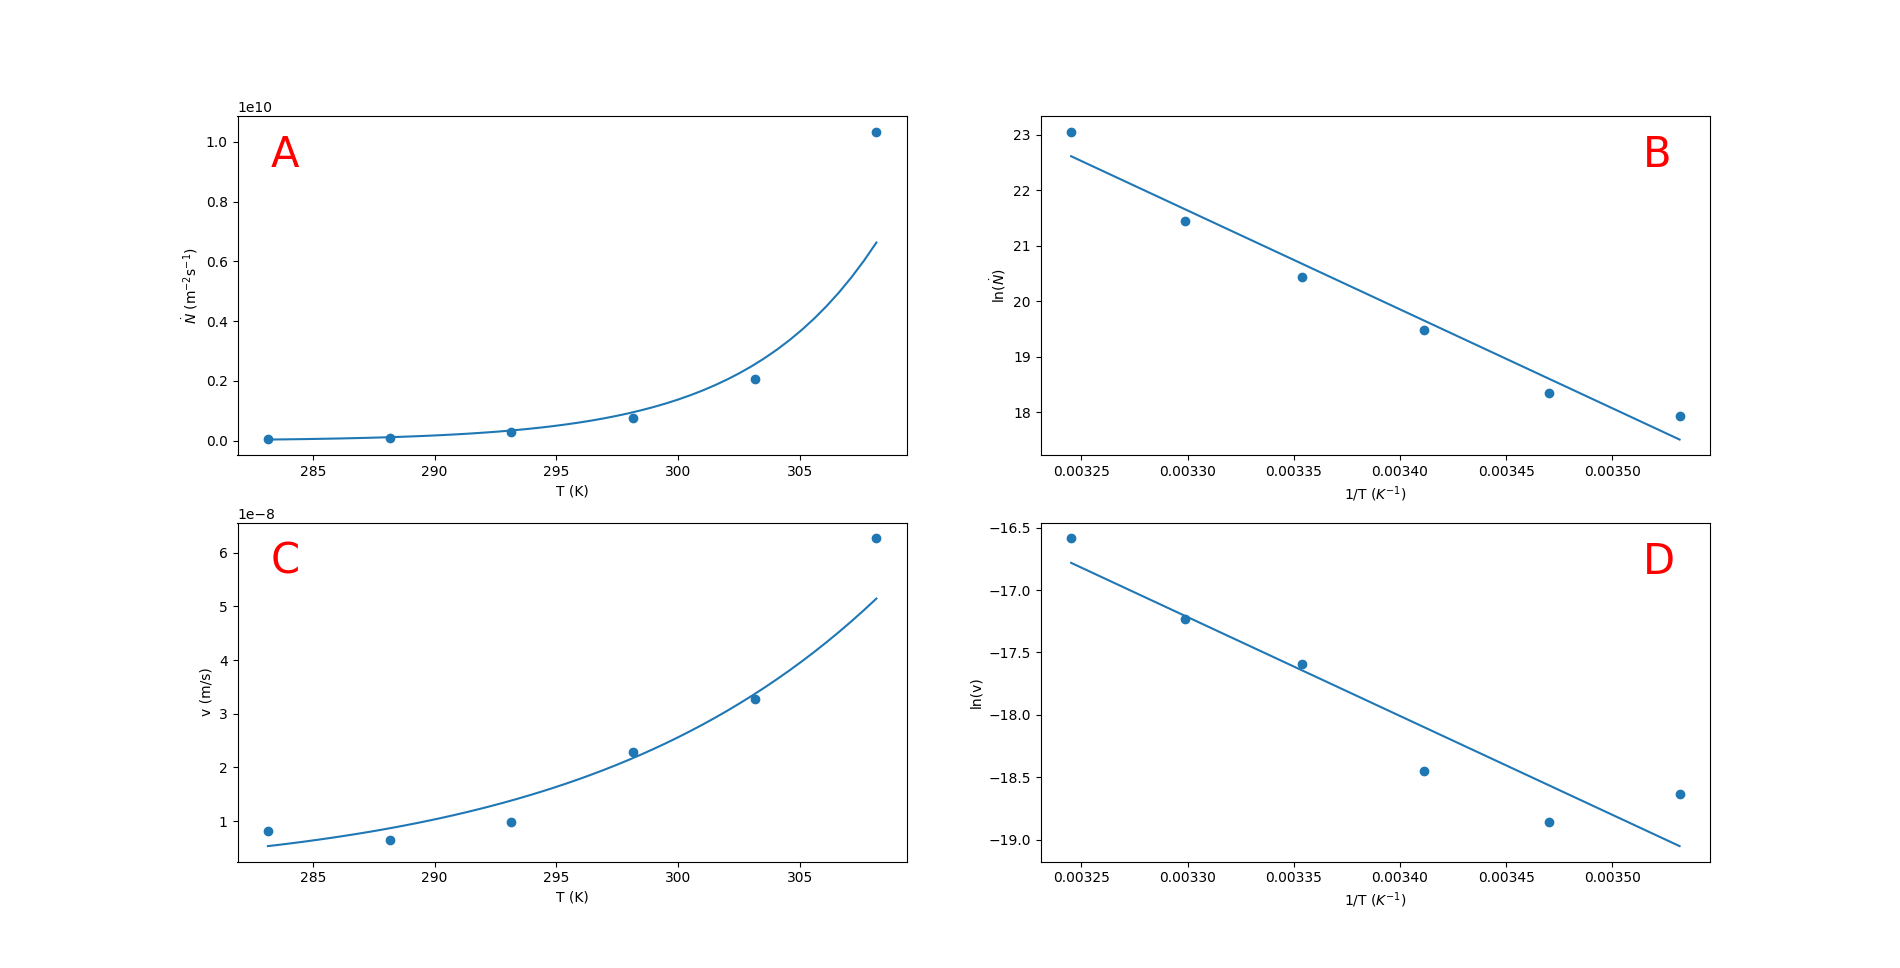
\includegraphics[width=1.0\linewidth]{linear_fits.png}
		\caption{}
		\label{fig:linear_fits}
	\end{figure}

Subtracting the activations energies yields the free energy change per atom of the critical nucleus, $\Delta G(ic) = 0.853$ eV, with a standard error of 0.696 eV.

The next logical step is to estimate the critical cluster size ($i_c$) and the enthalpy of crystallization ($-g_{c \rightarrow a}$); however this requires knowledge of the $\gamma$-factor that appears in Equation \ref{eqn:deltaG}.  An extremely-loose estimate may be obtained by the Materials Project: the average surface free energy of a Te Wulff crystal ($\gamma_s = 0.11 J/m^2$) may be taken as an upper bound for the possible energy of the crystalline-amorphous interface.

In order to convert from this surface free energy to the $\gamma$-factor of Equation \ref{eqn:deltaG}, a spherical critical nucleus is assumed, for which the nucleation barrier is typically calculated in terms of the critical radius ($r_c$):

\begin{equation}
	\Delta G(r_c) = -\frac{4}{3}\pi r_c^3 \Delta G_v + 4 \pi r_c^2 \gamma_s
	\label{eqn:rc}
\end{equation}

Recognizing that $V_c = \frac{4}{3}\pi r_c^3 = \Omega i_c$ where the atomic volume $\Omega = 35.031$ $\si{\angstrom}^3$, the expression $r_c = \left( \frac{3\Omega i_c}{4\pi} \right)^{1/3}$ may be obtained, yielding the following alternate form of Equation \ref{eqn:rc}:

\begin{equation}
	\Delta G(r_c) = -\Delta G_v \Omega i_c + 4 \pi \gamma_s \left( \frac{3\Omega i_c}{4\pi} \right)^{2/3} 
	\label{eqn:rc_ic}
\end{equation}

A comparison with Equation \ref{eqn:deltaG} reveals that the desired $\gamma$-factor may be calculated as $\gamma = 4 \pi \gamma_s \left( \frac{3\Omega}{4\pi} \right)^{2/3}$.  Recalling that the free energy of the spherical critical nucleus may be expressed as $\Delta G(i_c) = \frac{4 \gamma^3}{27 g^2_{c \rightarrow a}}$, the energy difference between amorphous and crystalline phases may be calculated as $g_{c \rightarrow a} = \sqrt{\frac{4 \gamma^3}{27 \Delta G(i_c)}}$, while the critical nucleus size is obtained as $i_c = \frac{2 \gamma}{3 g_{c \rightarrow a}}$.

Following these equations, the upper surface energy limit of $\gamma_s = 0.11 J/m^2$ yields $\gamma = 0.356$ eV, $g_{c \rightarrow a} = 0.088$ eV, and a critical cluster size $i_c = 2.683$ atoms.  By design, these values represent a lower limit; the critical cluster size may be made arbitrarily large by decreasing the estimate of $\gamma$ towards 0 eV.  This relationship is illustrated in Figure \ref{fig:cluster_size}.

	\begin{figure}[h]
		\centering
		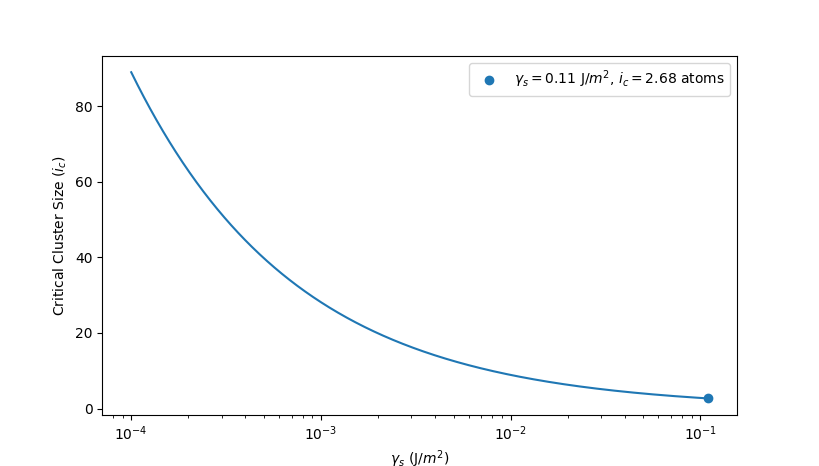
\includegraphics[width=1.0\linewidth]{cluster_size.png}
		\caption{}
		\label{fig:cluster_size}
	\end{figure}
